\likeechapter{Приложение B}
\appendix
\counterwithout{figure}{chapter}
\setcounter{figure}{0}
\begin{figure}[H]
	\centering
	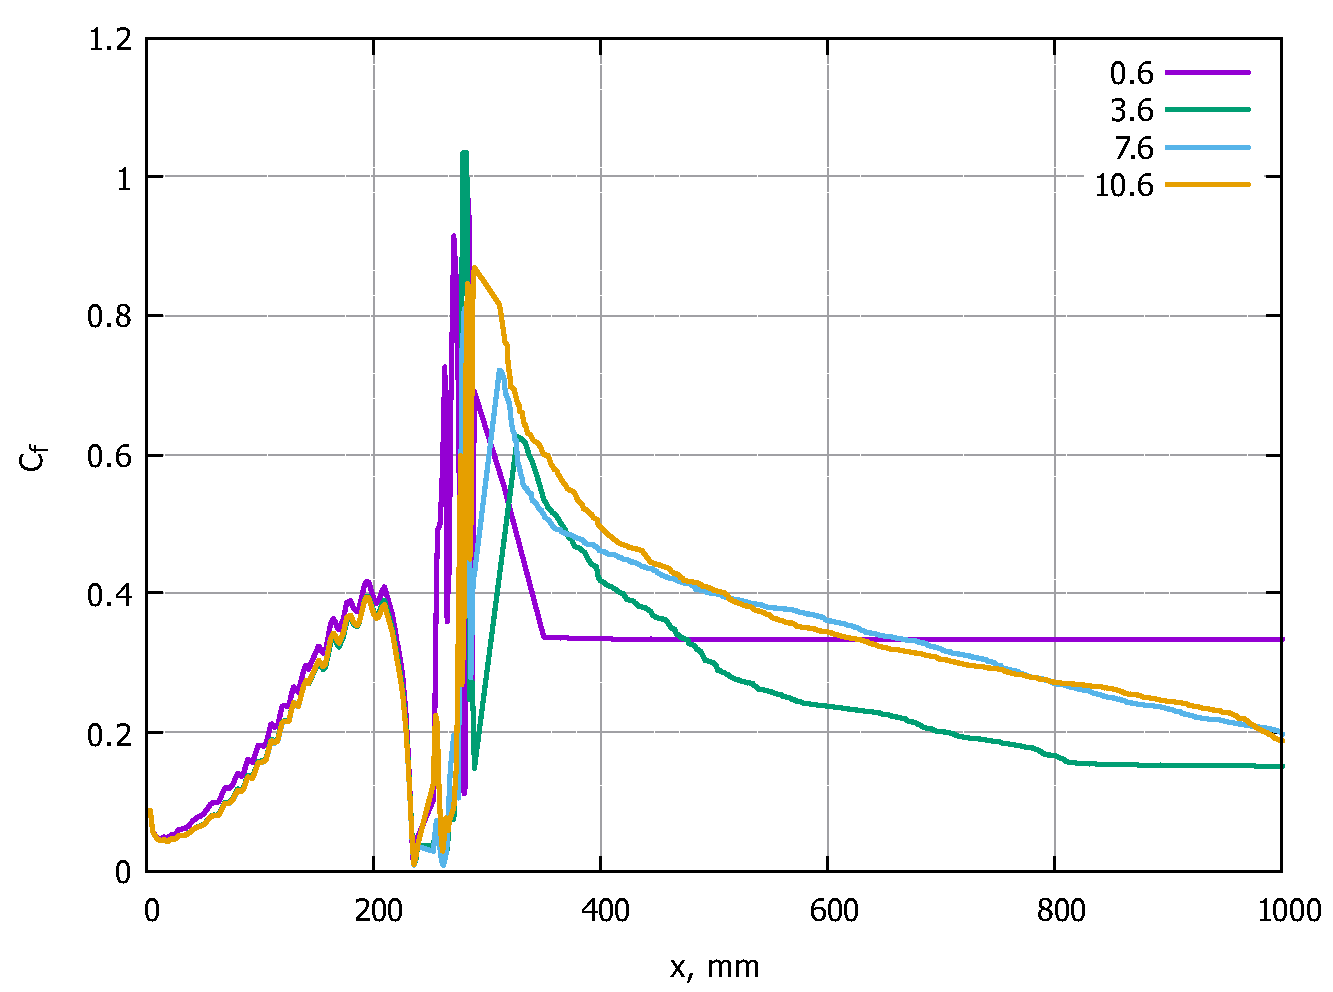
\includegraphics[width=0.8\linewidth]{../Assets/Cf-Tall}
	\caption{Изменение коэффициента трения по длине канала, z = 0}
	\label{fig:cf-tall}
\end{figure}
\begin{figure}[H]
	\centering
	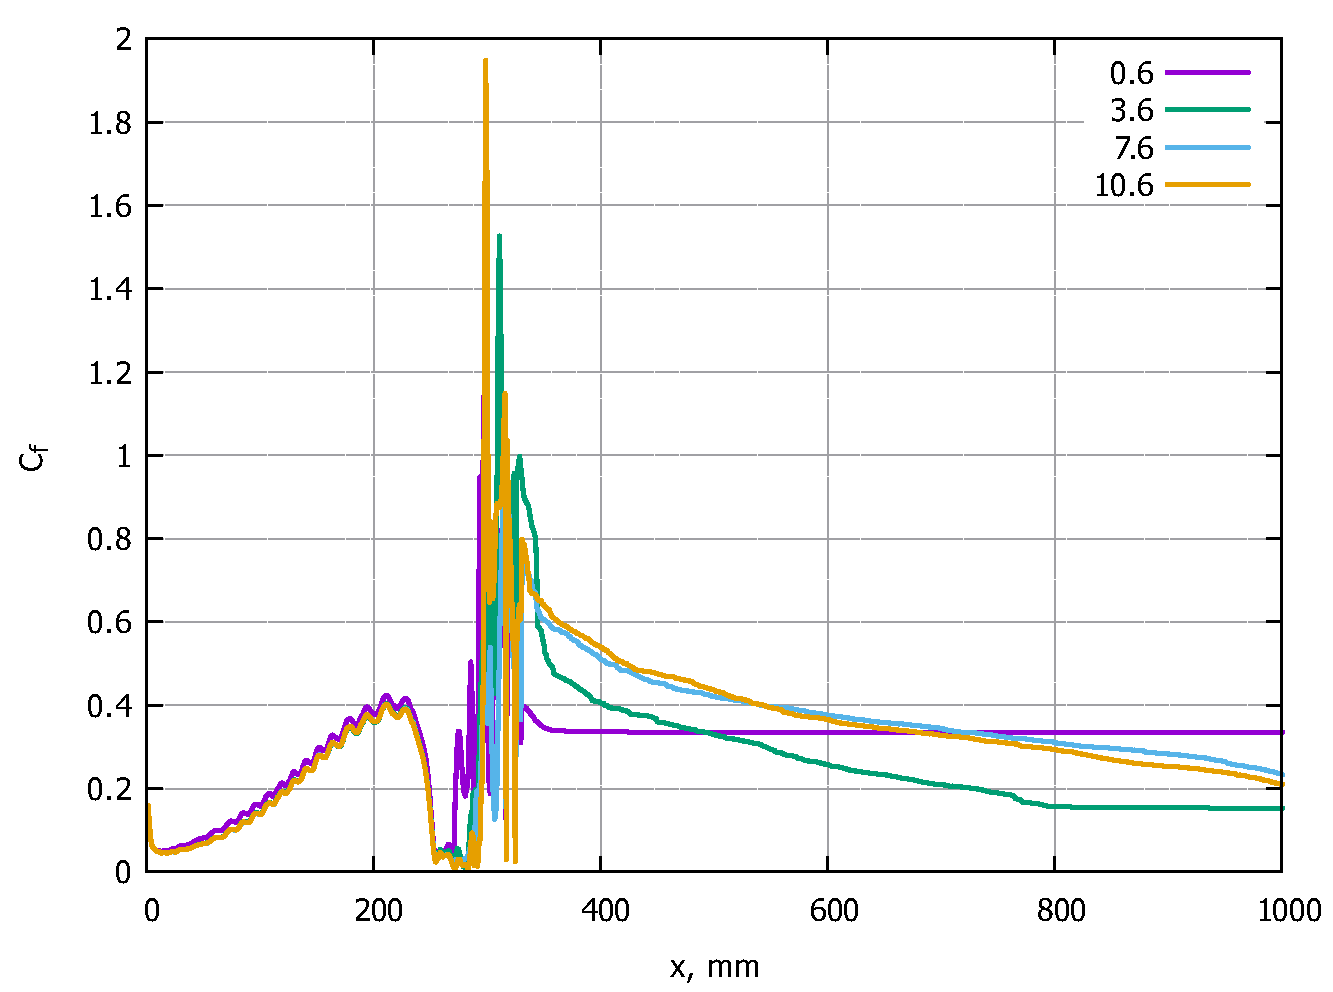
\includegraphics[width=0.8\linewidth]{../Assets/Cf-Tall-31m}
	\caption{Изменение коэффициента трения по длине канала, z = -31}
	\label{fig:cf-tall-31m}
\end{figure}
\newpage
\begin{flushright}
	\MakeUppercase{\textbf{Приложение B}}
\end{flushright}
\begin{figure}[H]
	\centering
	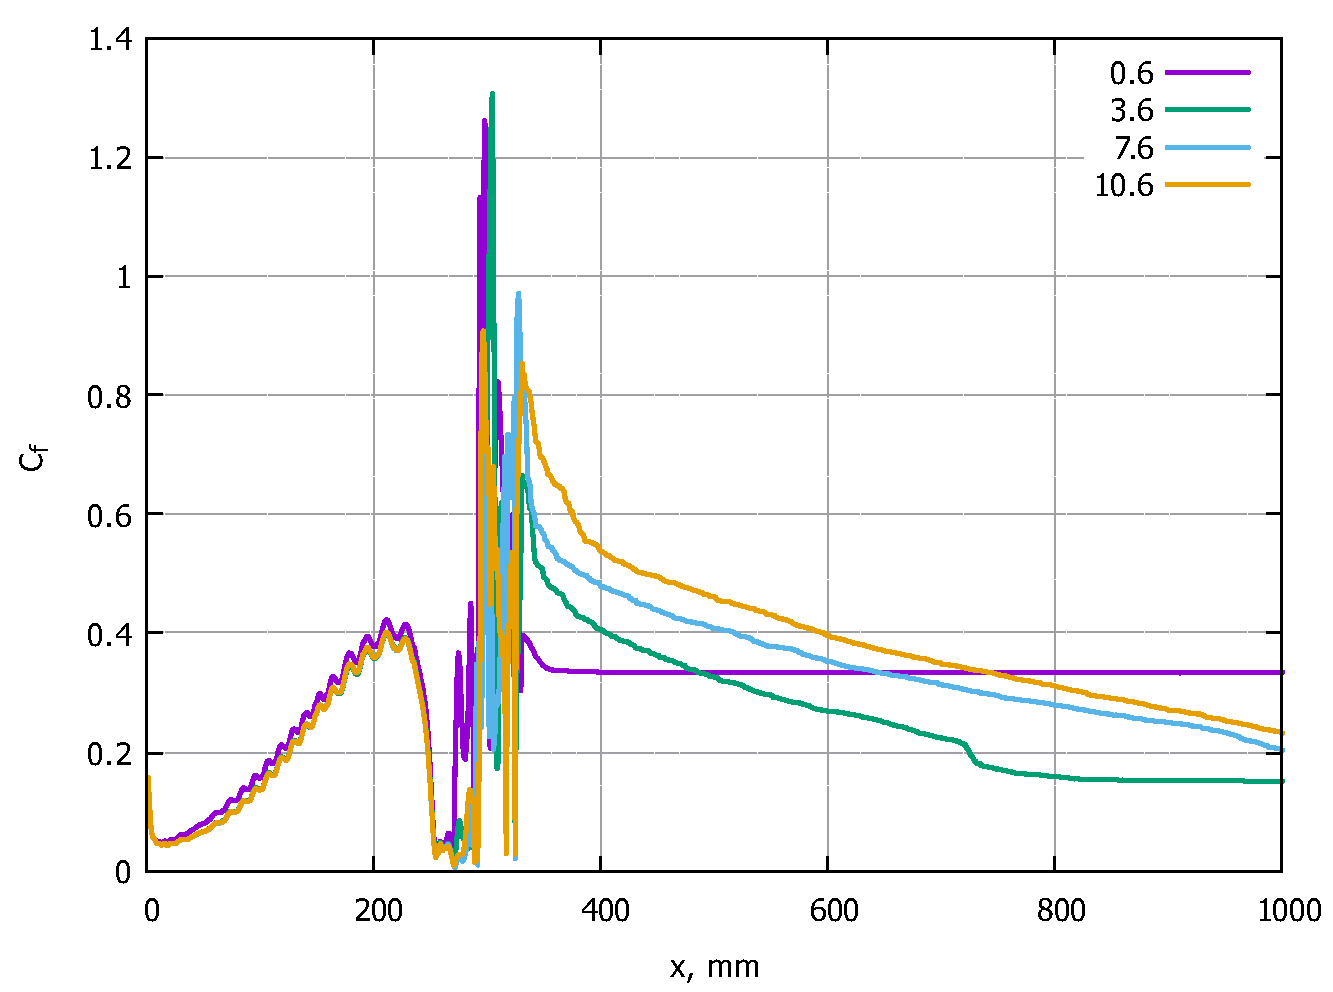
\includegraphics[width=0.8\linewidth]{../Assets/Cf-Tall-31p}
	\caption{Изменение коэффициента трения по длине канала, z = 31}
	\label{fig:cf-tall-31p}
\end{figure}
\begin{figure}[H]
	\centering
	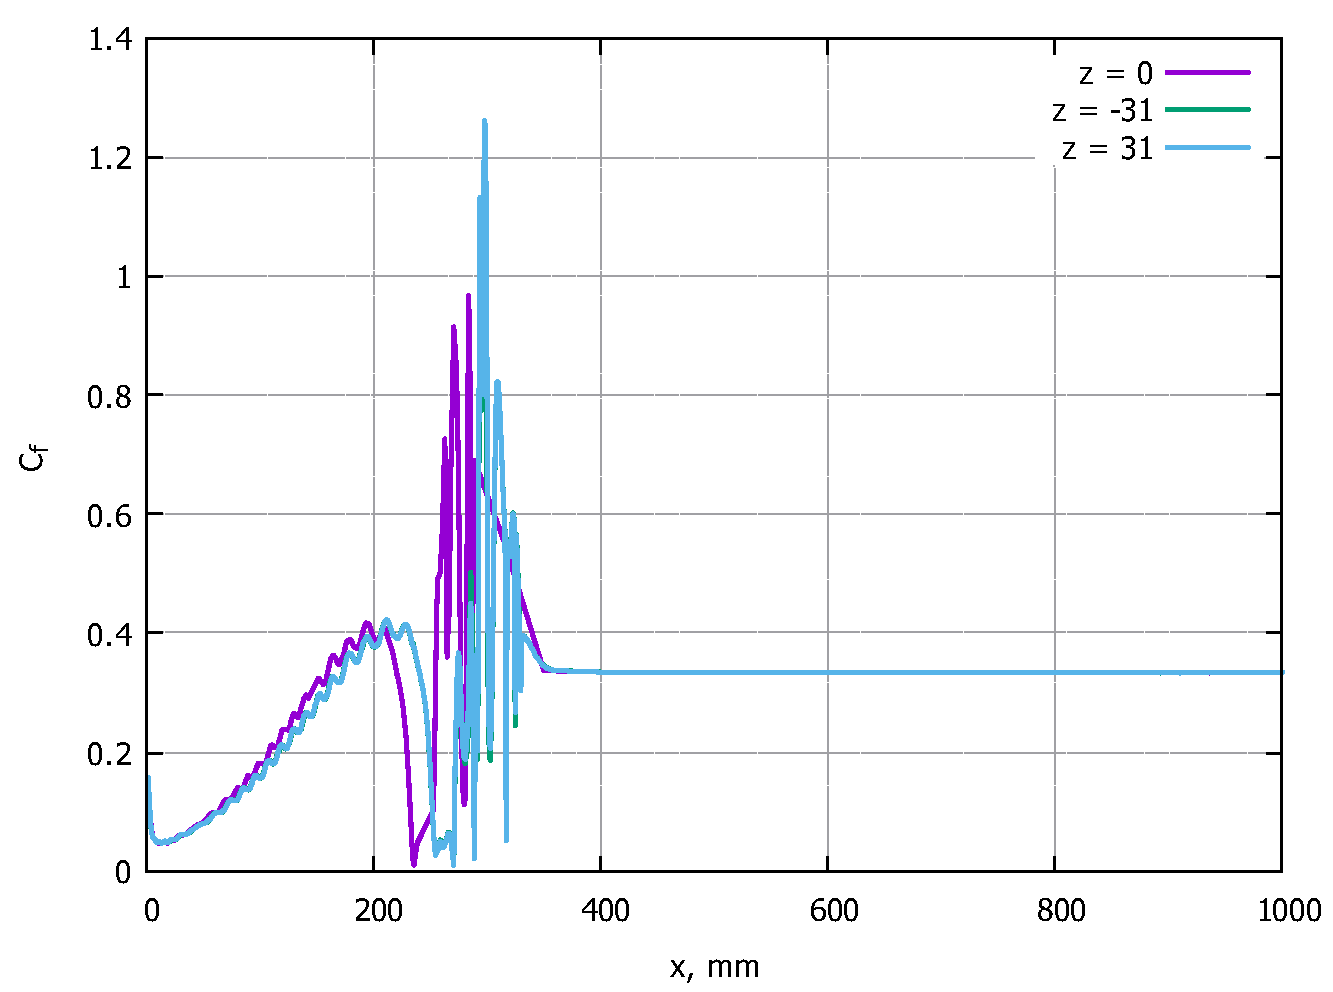
\includegraphics[width=0.8\linewidth]{../Assets/Cf-T06-all}
	\caption{Изменение коэффициента трения по длине канала, t = 0.6}
	\label{fig:cf-t06-all}
\end{figure}
\newpage
\begin{flushright}
	\MakeUppercase{\textbf{Приложение B}}
\end{flushright}
\begin{figure}[H]
	\centering
	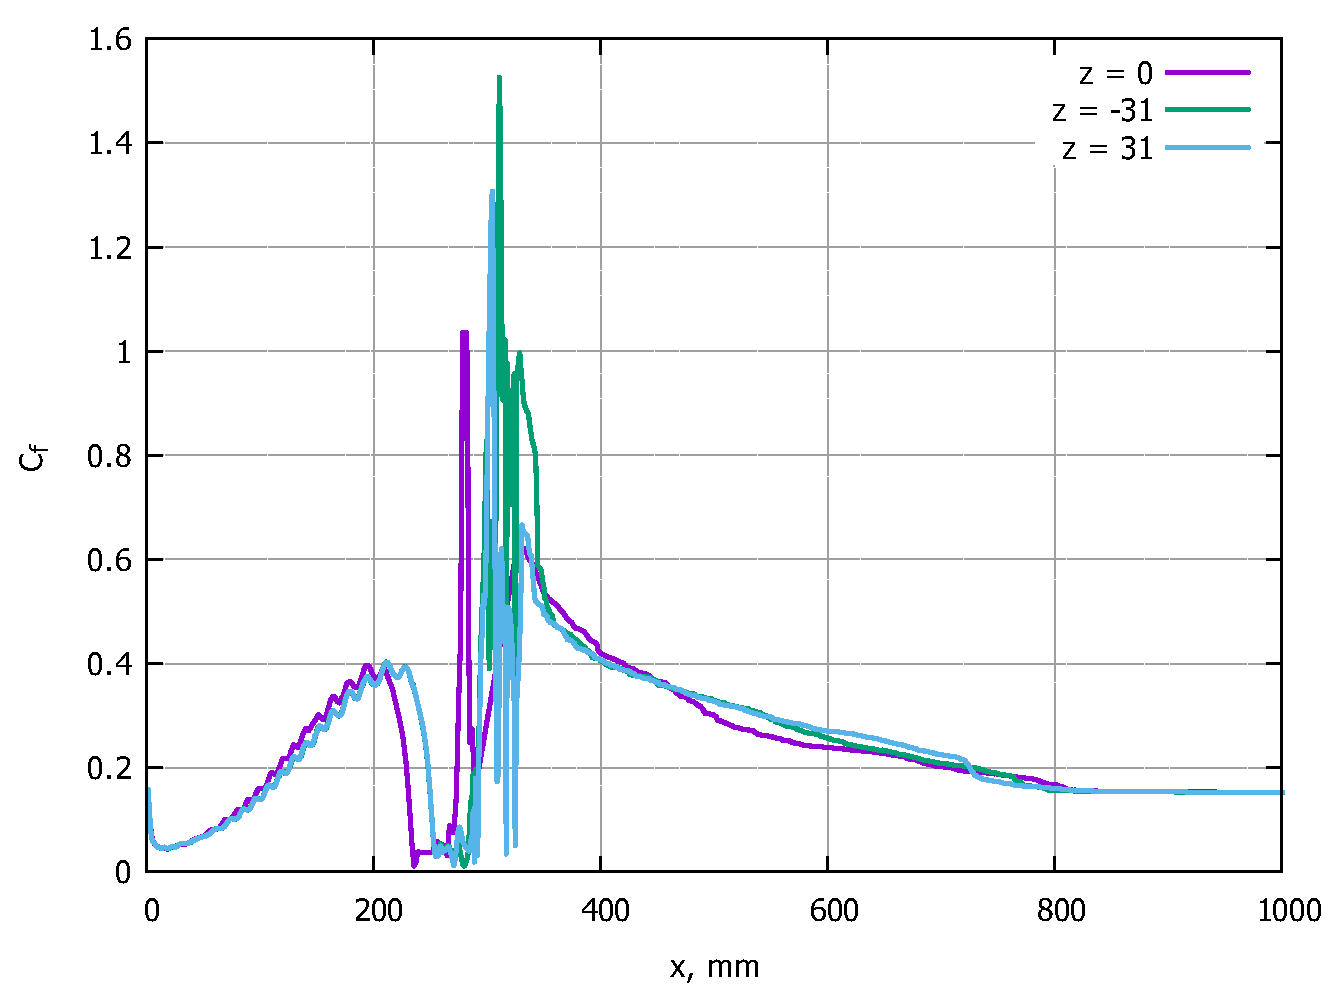
\includegraphics[width=0.8\linewidth]{../Assets/Cf-T360-all}
	\caption{Изменение коэффициента трения по длине канала, t = 3.6}
	\label{fig:cf-t360-all}
\end{figure}
\begin{figure}[H]
	\centering
	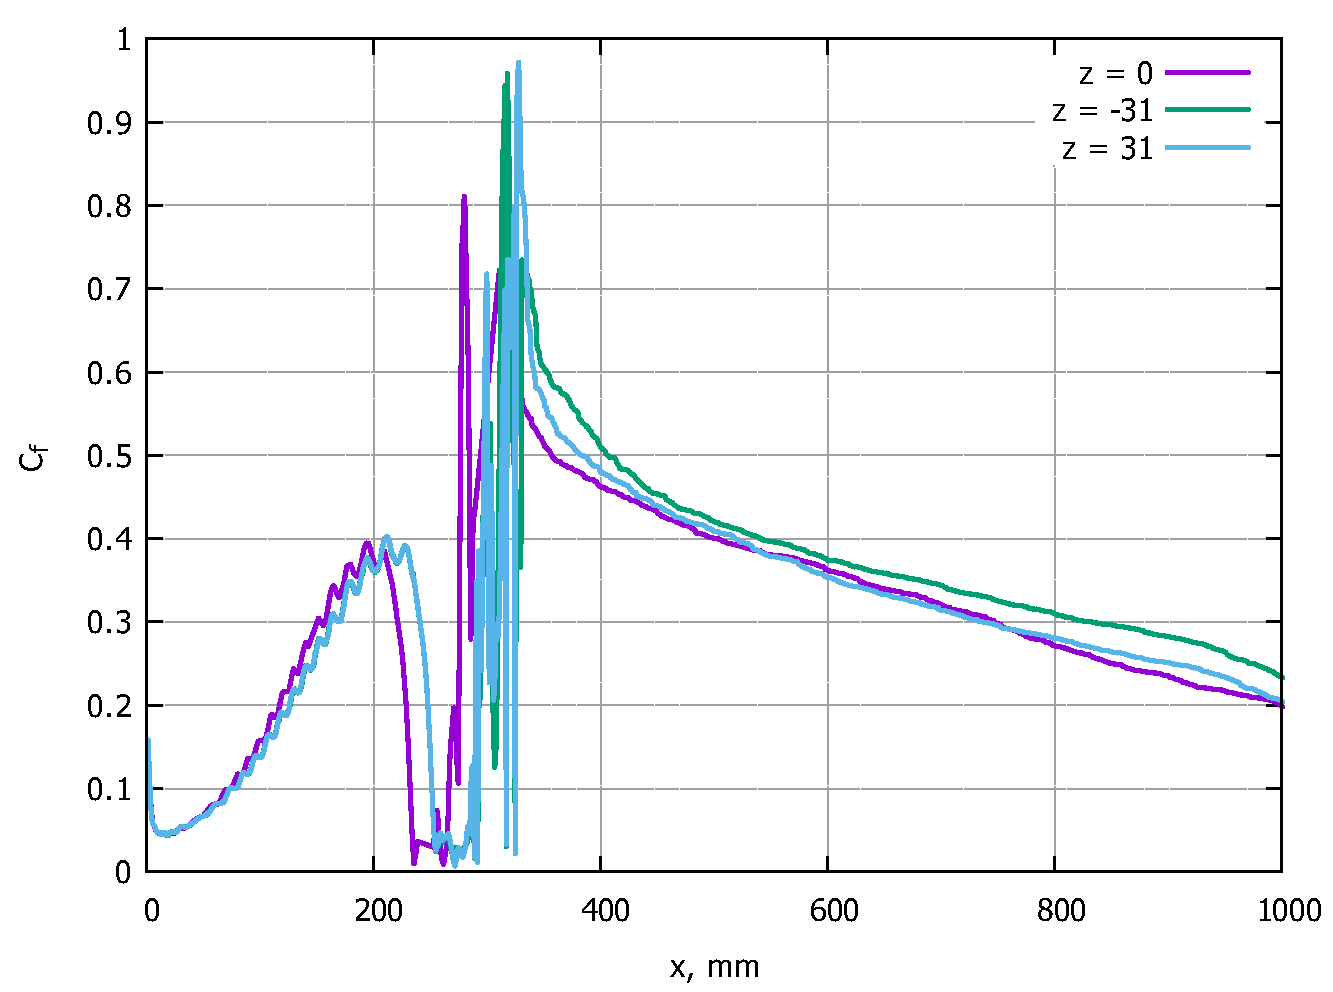
\includegraphics[width=0.8\linewidth]{../Assets/Cf-T760-all}
	\caption{Изменение коэффициента трения по длине канала, t = 7.6}
	\label{fig:cf-t760-all}
\end{figure}
\newpage
\begin{flushright}
	\MakeUppercase{\textbf{Приложение B}}
\end{flushright}
\begin{figure}[H]
	\centering
	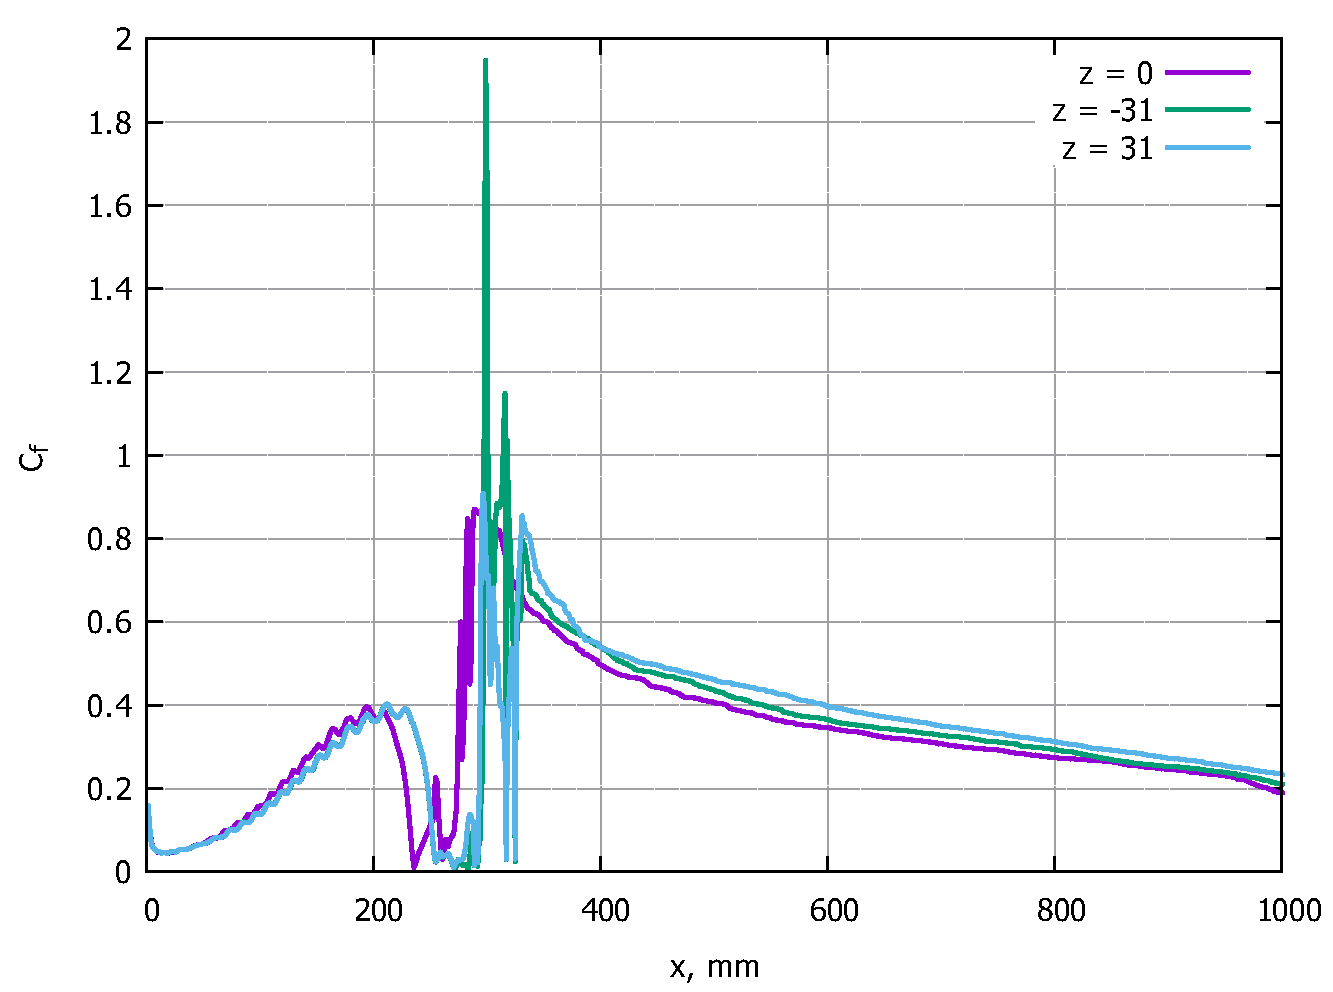
\includegraphics[width=0.8\linewidth]{../Assets/Cf-T1060-all}
	\caption{Изменение коэффициента трения по длине канала, t = 10.6}
	\label{fig:cf-t1060-all}
\end{figure}
